\documentclass[11pt,a4paper]{article}

\usepackage[utf8]{inputenc}
\usepackage[T1]{fontenc}
\usepackage[margin=1in]{geometry}
\usepackage{amsmath,amssymb,amsfonts}
\usepackage{graphicx}
\usepackage{xcolor}
\usepackage{booktabs}
\usepackage{tabularx}
\usepackage{array}
\usepackage{listings}
\usepackage{tikz}
\usetikzlibrary{shapes.geometric, arrows.meta, positioning, calc, fit}
\usepackage{enumitem}
\usepackage{caption}
\usepackage{subcaption}
\usepackage{float}
\usepackage{hyperref}

\hypersetup{
    colorlinks=true,
    linkcolor=black,
    citecolor=black,
    urlcolor=blue!70!black,
    pdftitle={RARP and BOOTP},
    pdfauthor={Subham Bhat}
}

\definecolor{codebg}{rgb}{0.96,0.96,0.96}
\definecolor{codeframe}{rgb}{0.25,0.25,0.25}
\definecolor{codenum}{rgb}{0.45,0.45,0.45}

\lstset{
    backgroundcolor=\color{codebg},
    basicstyle=\ttfamily\footnotesize,
    breakatwhitespace=false,
    breaklines=true,
    captionpos=b,
    commentstyle=\color{codenum}\itshape,
    keywordstyle=\bfseries,
    numberstyle=\tiny\color{codenum},
    numbers=left,
    numbersep=8pt,
    frame=single,
    rulecolor=\color{codeframe},
    tabsize=4,
    columns=flexible,
    keepspaces=true,
    showspaces=false,
    showstringspaces=false,
    xleftmargin=14pt,
    xrightmargin=4pt,
    literate={→}{{$\rightarrow$}}1 {←}{{$\leftarrow$}}1 {–}{{--}}1 {—}{{---}}1 {·}{{$\cdot$}}1 {✓}{{OK}}2 {✗}{{X}}1
}

\newcolumntype{Y}{>{\raggedright\arraybackslash}X}

% screenshot from docs/screenshots (skipped quietly if the file is missing)
\newcommand{\shot}[3][0.92\textwidth]{%
  \IfFileExists{docs/screenshots/#2}{%
  \begin{figure}[H]\centering
  \includegraphics[width=#1,keepaspectratio]{docs/screenshots/#2}
  \caption{#3}\end{figure}}{}}

\emergencystretch=3em
\setlength{\parindent}{1.5em}
\setlength{\parskip}{0.4em}

\begin{document}

% ==============================================================================
% TITLE PAGE
% ==============================================================================
\begin{titlepage}
    \centering
    \vspace*{4.2cm}

    {\LARGE \textbf{Before DHCP: RARP on a Simulated Ethernet}}\\[0.7em]
    {\LARGE \textbf{and BOOTP over UDP with a Relay Agent}}\\[0.7em]
    {\LARGE \textbf{(RFC 903, RFC 951, RFC 1542)}}\\[1.4em]

    {\large for Computer Networks Laboratory}

    \vspace{3.8cm}

    {\large
    \textbf{Name:} Subham Bhat\\[0.55em]
    \textbf{Class:} BCSE III\\[0.55em]
    \textbf{Roll:} 002410501020\\[0.55em]
    \textbf{Group:} A1\\[0.55em]
    \textbf{College:} Jadavpur University
    }

    \vfill
    {\normalsize 1}
\end{titlepage}

% ==============================================================================
% TABLE OF CONTENTS
% ==============================================================================
\pagenumbering{roman}
\setcounter{page}{2}
\tableofcontents
\newpage

% ==============================================================================
% MAIN CONTENT
% ==============================================================================
\pagenumbering{arabic}
\setcounter{page}{3}

\section{Introduction}
\noindent A \textbf{diskless workstation} boots from a ROM on its network card. The ROM knows the card's MAC address, but nothing else: no IP address, no subnet mask, no router, and no file to boot. Before it can load an operating system over the network, the machine must ask someone for this configuration. Two protocols solved this before DHCP existed, and DHCP is built directly on the second:
\begin{itemize}[leftmargin=2em]
    \item \textbf{RARP} (Reverse ARP, \textbf{RFC 903}, 1984) reuses the ARP packet with new opcodes: ``my MAC is X, what is my IP?''. It runs directly on Ethernet (EtherType \texttt{0x8035}), so its broadcast \textbf{cannot cross a router}, and the answer is \emph{only} an IP address.
    \item \textbf{BOOTP} (Bootstrap Protocol, \textbf{RFC 951}, 1985) runs over \textbf{UDP} (server port 67, client port 68). One reply carries the IP address, the boot server, the \textbf{boot file name}, and options such as mask, router and DNS (RFC 1497). A \textbf{relay agent} on the router (RFC 1542) forwards requests across subnets using the \texttt{giaddr} field.
\end{itemize}
In both protocols every address is fixed per MAC in a table typed in by an administrator; there are no pools and no leases. DHCP (1993) kept the BOOTP message, ports and relay mechanism and added dynamic allocation.

\subsection{What Was Built}
This module reproduces both protocols in pure Java 11 with no external libraries:
\begin{enumerate}[leftmargin=2em]
    \item \textbf{RARP on a simulated Ethernet} with two LANs joined by a router: real 60-byte RARP frames (EtherType \texttt{0x8035}, opcodes 3 and 4), broadcast to every station, and a RARP server with an \texttt{/etc/ethers} table.
    \item \textbf{BOOTP over real UDP}: the 300-byte message, a server with an \texttt{/etc/bootptab} table, a client with retries and back-off, and a \textbf{relay agent} that can be switched off.
    \item \textbf{A step-by-step simulation} on \texttt{http://localhost:8085}: every frame and packet is animated on the network drawing and can be opened byte by byte.
\end{enumerate}

\begin{table}[H]
\centering
\caption{The lab network}
\small
\begin{tabularx}{\textwidth}{@{}llY@{}}
\toprule
\textbf{Station} & \textbf{Where} & \textbf{Role} \\ \midrule
Boot server & LAN A, 10.0.1.5 & RARP server (\texttt{/etc/ethers}) and BOOTP server (\texttt{/etc/bootptab}), also the TFTP boot server \\
Router & 10.0.1.1 (LAN A), 10.0.2.1 (LAN B) & Joins the two LANs; optionally runs the BOOTP relay agent \\
WS-1 & LAN A & Diskless, registered: 10.0.1.21 \\
WS-4 & LAN B & Diskless, registered: 10.0.2.24, but on the far side of the router \\
WS-3 & LAN A & Diskless, not registered: the server stays silent \\ \bottomrule
\end{tabularx}
\end{table}

\begin{table}[H]
\centering
\caption{Ports (BOOTP uses non-privileged copies of 67/68 so that it runs without administrator rights)}
\small
\begin{tabular}{@{}lll@{}}
\toprule
\textbf{Port} & \textbf{Real port} & \textbf{Role} \\ \midrule
UDP 1067 & 67 & BOOTP server \\
UDP 2067 & 67 (on the router) & Relay agent \\
UDP 1068 & 68 & BOOTP client \\
HTTP 8085 & & Dashboard \\ \bottomrule
\end{tabular}
\end{table}

\shot{01_before_dhcp.png}{The dashboard: the two-LAN network with the boot server, the router and the diskless workstations.}

% ==============================================================================
\section{Packet Formats}

\subsection{The RARP Frame}
RARP uses exactly the 28-byte ARP payload. Only the EtherType and the opcodes differ. Because the sender does not know its own IP address, the protocol fields are zero in the request, and the requester's MAC appears both as sender and as target hardware address.

\begin{table}[H]
\centering
\caption{RARP frame (60 bytes on the wire, padded to the Ethernet minimum)}
\small
\begin{tabularx}{\textwidth}{@{}llY@{}}
\toprule
\textbf{Bytes} & \textbf{Field} & \textbf{Value in a request} \\ \midrule
0--5 & Destination MAC & \texttt{ff:ff:ff:ff:ff:ff} (broadcast) \\
6--11 & Source MAC & the workstation's MAC \\
12--13 & EtherType & \texttt{0x8035} = RARP (ARP is \texttt{0x0806}) \\
14--15, 16--17 & HTYPE, PTYPE & 1 = Ethernet, \texttt{0x0800} = IPv4 \\
18, 19 & HLEN, PLEN & 6, 4 \\
20--21 & OPER & 3 = reverse request, 4 = reverse reply \\
22--27, 28--31 & SHA, SPA & own MAC, 0.0.0.0 \\
32--37, 38--41 & THA, TPA & own MAC, 0.0.0.0 (in the reply: TPA = the assigned IP) \\
42--59 & padding & zeros \\ \bottomrule
\end{tabularx}
\end{table}

\begin{lstlisting}[language=Java, caption={Building a RARP frame (\texttt{rarp/Rarp.java}).}]
public static final int ETH_ARP = 0x0806, ETH_RARP = 0x8035;
public static final int REQUEST = 3, REPLY = 4;

public static byte[] frame(String dst, String src, int op, String sha, String spa, String tha, String tpa) {
    byte[] f = new byte[60];                                  // zero padding to 60 bytes
    System.arraycopy(Field.macBytes(dst), 0, f, 0, 6);
    System.arraycopy(Field.macBytes(src), 0, f, 6, 6);
    f[12] = (byte) (ETH_RARP >> 8); f[13] = (byte) ETH_RARP;  // EtherType 0x8035
    f[14] = 0; f[15] = 1;                                      // HTYPE 1 = Ethernet
    f[16] = 0x08; f[17] = 0x00;                                // PTYPE 0x0800 = IPv4
    f[18] = 6; f[19] = 4;                                      // HLEN, PLEN
    f[20] = 0; f[21] = (byte) op;                              // 3 = request, 4 = reply
    System.arraycopy(Field.macBytes(sha), 0, f, 22, 6);
    System.arraycopy(Field.ipBytes(spa), 0, f, 28, 4);
    System.arraycopy(Field.macBytes(tha), 0, f, 32, 6);
    System.arraycopy(Field.ipBytes(tpa), 0, f, 38, 4);
    return f;
}
\end{lstlisting}

\subsection{The BOOTP Message}
A BOOTP message is always 300 bytes: a 236-byte fixed part and a 64-byte vendor area. The vendor area begins with the \textbf{magic cookie} 99.130.83.99 (\texttt{63 82 53 63}), followed by options in type-length-value form. DHCP uses exactly the same layout and cookie and adds option 53 (message type).

\begin{table}[H]
\centering
\caption{BOOTP message fields (RFC 951)}
\small
\begin{tabularx}{\textwidth}{@{}llY@{}}
\toprule
\textbf{Offset} & \textbf{Field} & \textbf{Meaning} \\ \midrule
0 & op & 1 = BOOTREQUEST, 2 = BOOTREPLY \\
1, 2, 3 & htype, hlen, hops & 1 (Ethernet), 6, number of relay agents passed \\
4 & xid (4) & Random transaction ID chosen by the client \\
8, 10 & secs, flags & Seconds since the client started trying \\
12 & ciaddr & Client IP, if it already knows it \\
16 & yiaddr & ``Your'' IP: the address assigned by the server \\
20 & siaddr & The boot (TFTP) server \\
24 & giaddr & The relay agent's address, if a relay forwarded the request \\
28 & chaddr (16) & Client hardware address \\
44 & sname (64) & Optional server host name \\
108 & file (128) & Boot file name, e.g.\ \texttt{/tftpboot/sunos-ws1.img} \\
236 & vend (64) & Magic cookie, then options: 1 mask, 3 router, 6 DNS, 12 host name, 255 end \\ \bottomrule
\end{tabularx}
\end{table}

\begin{lstlisting}[language=Java, caption={Encoding the 300-byte BOOTP message (\texttt{bootp/Packet.java}).}]
public byte[] encode() {
    byte[] b = new byte[SIZE];                                   // SIZE = 300
    b[0] = (byte) op; b[1] = 1; b[2] = 6; b[3] = (byte) hops;
    b[4] = (byte) (xid >> 24); b[5] = (byte) (xid >> 16); b[6] = (byte) (xid >> 8); b[7] = (byte) xid;
    b[8] = (byte) (secs >> 8); b[9] = (byte) secs; b[10] = (byte) (flags >> 8); b[11] = (byte) flags;
    put(b, 12, Field.ipBytes(ciaddr)); put(b, 16, Field.ipBytes(yiaddr));
    put(b, 20, Field.ipBytes(siaddr)); put(b, 24, Field.ipBytes(giaddr));
    put(b, 28, Field.macBytes(chaddr));
    str(b, 44, 64, sname); str(b, 108, 128, file);
    put(b, 236, COOKIE);                                         // 99.130.83.99
    int p = 240;
    for (Map.Entry<Integer, byte[]> o : options.entrySet()) {     // type, length, value
        if (p + 2 + o.getValue().length >= SIZE) break;
        b[p++] = (byte) (int) o.getKey(); b[p++] = (byte) o.getValue().length;
        put(b, p, o.getValue()); p += o.getValue().length;
    }
    b[p] = (byte) OPT_END;
    return b;
}
\end{lstlisting}

\shot[0.85\textwidth]{05_bootp_packet.png}{A BOOTREPLY opened byte by byte: yiaddr, siaddr, the boot file, the magic cookie and the options.}

% ==============================================================================
\section{System Architecture}

\begin{figure}[H]
\centering
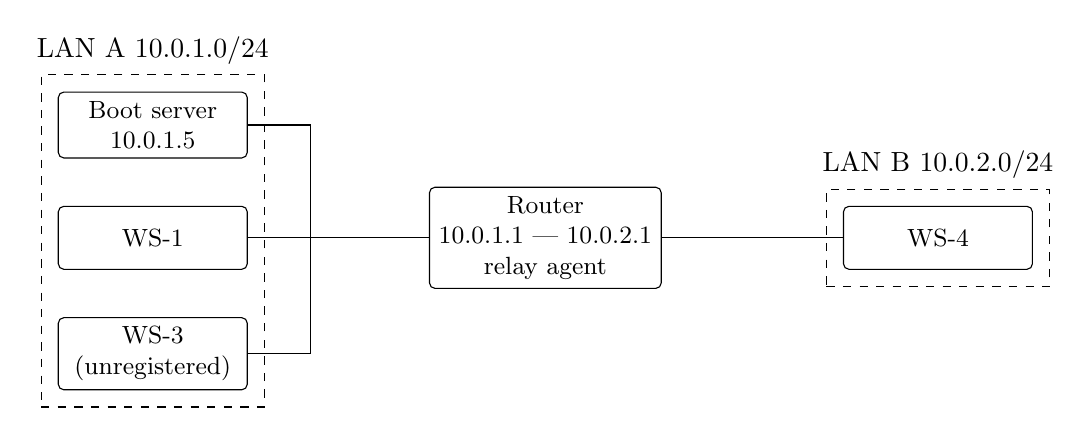
\begin{tikzpicture}[node distance=0.6cm, box/.style={draw, rounded corners=2pt, minimum width=2.4cm, minimum height=0.8cm, align=center, font=\small}, >=Stealth]
\node[box] (srv) {Boot server\\10.0.1.5};
\node[box, below=of srv] (ws1) {WS-1};
\node[box, below=of ws1] (ws3) {WS-3\\(unregistered)};
\node[box, right=2.3cm of ws1] (rt) {Router\\10.0.1.1 | 10.0.2.1\\relay agent};
\node[box, right=2.3cm of rt] (ws4) {WS-4};
\node[draw, dashed, fit=(srv)(ws1)(ws3), inner sep=6pt, label=above:{LAN A 10.0.1.0/24}] {};
\node[draw, dashed, fit=(ws4), inner sep=6pt, label=above:{LAN B 10.0.2.0/24}] {};
\draw (srv.east) -- ++(0.8,0) |- (rt.west); \draw (ws1.east) -- (rt.west); \draw (ws3.east) -- ++(0.8,0) |- (rt.west);
\draw (rt.east) -- (ws4.west);
\end{tikzpicture}
\caption{The simulated network: the boot server is on LAN A; WS-4 is on the far side of the router.}
\end{figure}

\begin{itemize}[leftmargin=2em]
    \item \texttt{rarp/Lan.java} simulates the two Ethernet segments: a broadcast is delivered to every station on the same segment, and the router does not forward it.
    \item \texttt{rarp/Rarp.java} builds and dissects RARP frames.
    \item \texttt{bootp/Packet.java} encodes and decodes BOOTP messages; \texttt{bootp/Bootp.java} runs the server, the relay agent and the client on real UDP sockets.
    \item \texttt{dashboard/DashboardServer.java} serves the step-by-step simulation; every event carries the bytes and a decoded field list.
\end{itemize}

% ==============================================================================
\section{Workflows and Observations}

\subsection{RARP on the Same LAN}
WS-1 broadcasts a RARP request (op 3). Every station on LAN A receives it; the router receives it too but does not forward it. The RARP server finds WS-1's MAC in \texttt{/etc/ethers} and sends a \textbf{unicast} reply (op 4) with TPA = 10.0.1.21. WS-1 now has an IP address, but still no mask, no router and no boot file; it would need further protocols to get them.

\shot[0.85\textwidth]{02_rarp_reply.png}{RARP on LAN A: broadcast request, unicast reply carrying only the IP address.}

\subsection{RARP Cannot Cross a Router}
WS-4 on LAN B broadcasts the same request. The router receives it and drops it, because link-layer broadcasts stop at routers, and RARP has no IP header that could be routed. The server on LAN A never hears it. WS-4 retries after 1 s, 2 s and 3 s, then gives up, even though the server has its MAC in the table. With RARP, every LAN needs its own server.

\shot[0.85\textwidth]{03_rarp_cannot_cross_router.png}{WS-4's RARP broadcast dies at the router; three retries, then failure.}

\subsection{BOOTP on the Same LAN}
WS-1 sends a BOOTREQUEST from \texttt{0.0.0.0:68} to \texttt{255.255.255.255:67}: op 1, its MAC in \texttt{chaddr}, a random \texttt{xid}, all addresses zero. The server finds the MAC in \texttt{/etc/bootptab} and returns a BOOTREPLY with \texttt{yiaddr} 10.0.1.21, boot server 10.0.1.5, boot file \texttt{/tftpboot/sunos-ws1.img}, and mask, router 10.0.1.1, DNS 10.0.1.53 and host name \texttt{ws1} in the vendor area. WS-1 matches \texttt{xid} and \texttt{chaddr} and configures itself; next it would download the boot file with TFTP. The binding is permanent: BOOTP has no leases.

\subsection{BOOTP Through the Relay Agent}
The relay agent on the router listens for BOOTREQUESTs on LAN B, writes its own LAN-B address into \texttt{giaddr}, increments \texttt{hops}, and forwards the request as a \textbf{unicast} UDP packet to the server. Because \texttt{giaddr} is set, the server sends the reply back to the relay, which delivers it on LAN B to port 68. The same \texttt{giaddr} also tells the server which subnet the client is on.

\begin{lstlisting}[language=Java, caption={The relay agent (\texttt{bootp/Bootp.java}).}]
Packet p = Packet.decode(buf, dp.getLength());
if (p.op == Packet.BOOTREQUEST) {
    if (!relayOn) { step(p.xid, "RELAY", "-", "dropped", "no relay agent: the broadcast dies at the router", null); continue; }
    if (p.hops >= 4) { step(p.xid, "RELAY", "-", "dropped", "hops limit reached, discarded", null); continue; }
    p.hops++;
    if (p.giaddr.equals("0.0.0.0")) p.giaddr = Topology.ROUTER_B_IP;   // 10.0.2.1
    byte[] out = p.encode();
    relay.send(new DatagramPacket(out, out.length, LO, SERVER_PORT));   // unicast to the server
} else {
    byte[] out = p.encode();                                           // BOOTREPLY coming back
    relay.send(new DatagramPacket(out, out.length, LO, CLIENT_PORT));  // deliver on LAN B, port 68
}
\end{lstlisting}

WS-4 receives 10.0.2.24 with router 10.0.2.1. With the relay agent switched off on the dashboard, the same request is dropped at the router, and WS-4 fails after three tries, exactly like RARP.

\shot[0.85\textwidth]{04_bootp_via_relay.png}{BOOTP through the relay: the forwarded request carries giaddr = 10.0.2.1 and hops = 1.}

\subsection{Unknown Machines}
WS-3 is not in either table. Both servers stay silent, because neither protocol has a pool of spare addresses; the client retries three times and gives up. Registering WS-3 from the dashboard's table and booting it again succeeds. This manual table is the main reason DHCP was introduced.

% ==============================================================================
\section{Verification and Results}

\begin{lstlisting}[language=bash, caption={Running the lab, the checks and the Python client.}]
cd RARP-BOOTP
run.bat                  # RARP LAN, BOOTP server + relay, dashboard (http://localhost:8085)
run.bat --verify         # 19 automated checks
python interop_test.py   # a BOOTREQUEST built by hand in Python against our server and relay (7 checks)
\end{lstlisting}

\begin{table}[H]
\centering
\caption{Verification checks (all 19 passed)}
\small
\begin{tabularx}{\textwidth}{@{}Y@{}}
\toprule
RARP frame is padded to the 60-byte Ethernet minimum; EtherType \texttt{0x8035}, not \texttt{0x0806}; payload is 28 bytes like ARP \\
Op 3 = reverse request with SHA = THA = own MAC and SPA = TPA = 0.0.0.0 \\
Request is a broadcast heard by every station on LAN A; reply is unicast (op 4) with TPA = 10.0.1.21 \\
Unregistered MAC: the server stays silent, three tries, then failure \\
WS-4 on LAN B fails with RARP: the router does not forward the broadcast \\
BOOTP message is always 300 bytes; round trip keeps xid, chaddr, yiaddr and file \\
Vendor area starts with the magic cookie 99.130.83.99; the subnet-mask option decodes \\
WS-1 gets IP 10.0.1.21 with mask, router, DNS, host name, boot server and boot file \\
WS-4 succeeds through the relay agent, which set giaddr = 10.0.2.1 and hops = 1 \\
Relay agent switched off: WS-4 fails, just like RARP \\ \bottomrule
\end{tabularx}
\end{table}

A BOOTREQUEST built byte by byte in Python, independently of our code, receives a correct BOOTREPLY both directly and through the relay agent (all 7 interoperation checks pass). A screen recording of the full simulation is in \texttt{docs/video}.

\begin{table}[H]
\centering
\caption{RARP, BOOTP and DHCP compared}
\small
\begin{tabularx}{\textwidth}{@{}lYYY@{}}
\toprule
 & \textbf{RARP} & \textbf{BOOTP} & \textbf{DHCP} \\ \midrule
Layer & Link (EtherType 0x8035) & UDP 67/68 & UDP 67/68 \\
Crosses routers & No & Yes, with a relay agent & Yes, with a relay agent \\
Gives & IP address only & IP, mask, router, DNS, boot file & All of BOOTP plus many options \\
Allocation & Static table & Static table & Pools, leases, renewal \\
Unknown client & No answer & No answer & Gets an address from the pool \\ \bottomrule
\end{tabularx}
\end{table}

\shot[0.8\textwidth]{06_lineage.png}{The lineage RARP $\rightarrow$ BOOTP $\rightarrow$ DHCP.}

% ==============================================================================
\section{Conclusion}
\begin{enumerate}[leftmargin=2em]
    \item \textbf{The layer decides the reach.} RARP lives directly on Ethernet, so its broadcast stops at the first router; BOOTP's move to UDP/IP made forwarding possible.
    \item \textbf{The relay agent is the key idea.} By catching the broadcast, writing its own address into \texttt{giaddr} and forwarding it as unicast, one central server can configure many subnets. DHCP uses the same mechanism unchanged.
    \item \textbf{Static tables do not scale.} Both protocols ignore unregistered machines and never reclaim addresses; DHCP kept the BOOTP message and added address pools and leases to solve exactly this.
\end{enumerate}

\section*{AI Acknowledgement}
\addcontentsline{toc}{section}{AI Acknowledgement}
Artificial Intelligence tools were used as an aid during this project. Specifically, AI assistance was used for:
\begin{itemize}[leftmargin=2em]
    \item \textbf{Protocol cross-checking:} comparing message formats, reply codes, state machines and byte offsets against the RFCs cited in this report.
    \item \textbf{Code review and testing:} suggesting edge cases for the automated verification suite and reviewing concurrency and error handling.
    \item \textbf{Writing and visualization:} drafting, structuring and refining the explanations, tables, diagrams and \LaTeX{} source of this report.
\end{itemize}
All protocol implementations, Java source code, experiments, measurements and final conclusions were run, reviewed and verified by the author, who takes full responsibility for the content of this report.

\end{document}
